\chapter{Часть 4}

\begin{textcitation}
	«Вернусь я к сыну и жене,
	и будут уж до с***и мне,
	арабы б****, арабы б****, арабы!»
\end{textcitation}

\textbf{Итак, мы пришли к самой важной части нашего рассказа. Непосредственно столкновению пилотов 1-й и 2-й эскадрилий советского 135-го истребительного авиаполка с израильскими лётчиками.}

{ \textbf{Сначала — несколько самых важных выводов:}
	\begin{itemize}
		\item в бою большую часть времени участвовали по 8 самолётов с каждой стороны, ещё 3 израильских присоединились на последнем этапе, и их появление не оказало особого влияния на исход. Ни одна из сторон не имела значительного количественного перевеса.
		\item эффект «внезапности» при появлении израильских самолётов был сильно преувеличен советской стороной, возможно, с целью оправдания собственного поражения.
		\item для израильтян, операция с самого начала пошла «не по плану». Фактический ход боя значительно отличался от изначально запланированного израильским командованием.
		\item 2 советских самолёта были сбиты в манёвренном бою, ещё 2— во время преследования выходящих из боя. Из «засады» не было сбито ни одного — израильтяне были обнаружены до начала атаки, а «Фантомы» были вынуждены вступить в манёвренный бой.
		
		\item главная причина поражения советской стороны - значительная разница в опыте советских и израильских лётчиков и их уровне готовности вести ближний манёвренный бой.
	\end{itemize}
\itshape}
\begin{remark}
	\textbf{Важный дисклеймер:}
	
	Представленная в статье версия того, как происходил знаменитый бой над Эль-Сохной (более известный под своим израильским кодовым названием операции — «Римон-20») не претендует на окончательность, полную достоверность и безошибочность. Тем не менее я считаю, что она является одной из наиболее близких к реальности из всех существующих в открытых источниках. Фактически она представляет собой попытку сопоставить множество израильских, советских и арабских описаний одного и того же боя. Часто эти описания противоречат друг другу — причем даже некоторые израильские не совпадают между собой, хотя они принадлежат лётчикам «братских» эскадрилий.
	
	Изначально ни одна из точек зрения и ни один из источников не был принят как достоверный. В случае противоречия подтверждение искалось в других источниках и в здравом смысле. Также я исходил из предположения, что каждая сторона лучше понимала процессы, происходившие на её стороне, и хуже — на стороне противника.
\end{remark}

Я старался использовать только первоисточники (т.е. воспоминания лётчиков и их современников), а не компиляции (статьи Заборского, Йоффе, и т.п.). Исключение составили книги людей, действительно имевших доступ к отчетам о том дне — «Призраки над Каиром» Дани Шалома и «Оспреевская» серия Шломо Алони, и отчасти — статья «Истребители в войне на истощение» Бабича.

Основой для статьи с израильской стороны послужили воспоминания ведущего четвёрки «Миражей-разведчиков» Амоса Амира из книги Fire in the sky, глава 29, дополненные цитатами из «Призраков над Каиром» (перевод Наума Шумбаева с моими дополнениями) и воспоминаниями Йифтаха Спектора, Коби Рихтера, Авиама Селы, Авиху Бен-Нуна, Авраама Салмона — из перечисленных выше книг, журнала ВВС Израиля и других источников. Использование всех из них позволило выстроить максимально точную картину.

\begin{figure}[h!tb] 
	\centering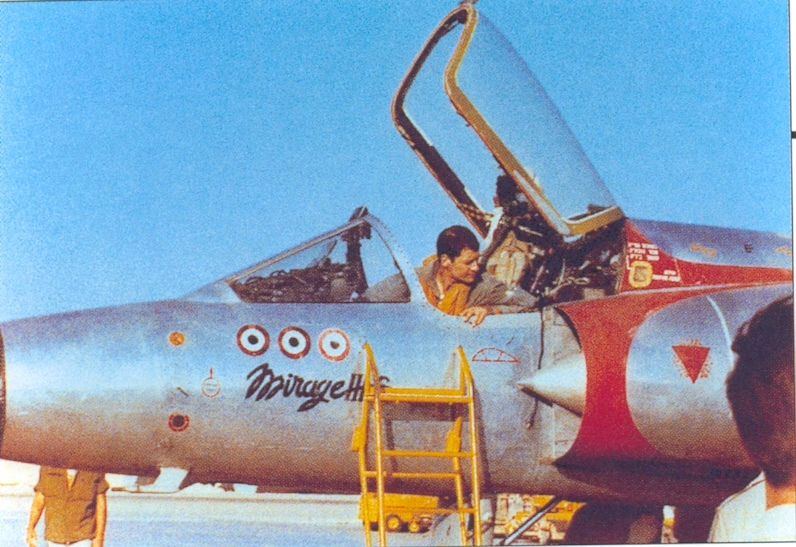
\includegraphics[scale=0.4]{Dolina_4/Avbi2GYLra4.jpg}
	%	\label{fig:scipion} % Unique label used for referencing the figure in-text\end{document}
	%	%\addcontentsline{toc}{figure}{Figure \ref{fig:placeholder}} % Uncomment to add the figure to the table of contents%----------------------------------------------------------------------------------------
	\caption{Спектор и его «Мираж», 1969 год}%	CHAPTER 2
\end{figure}

С советской стороны основой стали воспоминания пилота 1-й эскадрильи 135-го ИАП А.В. Акименкова, известного лётчика-испытателя, из его книги «На пороге иного мира», и В.Б. Ельчанинова из того-же 135-го ИАП из книги «Дан приказ ему в Египет». Дополнено отрывками из воспоминаний Васильева (лётчик 135-го ИАП), Рыболовлева (начальник группы объективного контроля Бени-Суэйф) и других.

Выражаю огромную признательность morelas, Науму Шумбаеву, и многим другим людям, чьими материалами я активно пользовался.

\section{Как это было (краткая версия)}

Утренний распорядок на аэродроме Бени-Суэф не менялся уже который день. Четвёрка заступает на утреннее дежурство в готовности №2, ближе к обеду их сменяют товарищи. У Канала вновь неспокойно — израильтяне бомбят египетские позиции, те в ответ стреляют. Советская авиация остаётся на аэродромах — израильтяне уже несколько месяцев как отказались от рейдов вглубь Египта. К середине дня израильские атаки заканчиваются, оставляя после себя огромные столбы дыма. Наступает тишина.

На советский КП докладывают: четвёрка «Скайхоков» атакует РЛС в районе Сохны, у самого канала. Поднимать авиацию смысла нет — к тому моменту, как советские самолёты окажутся у Канала, израильтяне уже будут у себя дома.

Казалось, это был ещё один скучный день — как вдруг над Синаем появилась отметка, похожая на транспортный самолёт. Через несколько кругов становится понятно — это израильский воздушный командный пункт управления авиацией. А ближе к Каналу замелькали отметки вертолётов. Зачем они здесь?...

Пока в Бир-Арейде и Бени-Суэф думали над происходящим, в небе начиналась прелюдия к грандиозному представлению. Четвёрка «Миражей» с авиабазы Рефидим взмыла в воздух. Они летели очень плотным строем — так, чтобы на радарах казаться парой самолётов — разведчиков. Отличная мишень: безоружная, наглая — и такая близкая! В их кабинах сидели пилоты самой результативной истребительной четвёрки ВВС Израиля, лучшие лётчики 119-й эскадрильи «Миражей».

Тем временем, над верхушками деревьев к Суэцкому заливу приближались другие актёры — четыре «Фантома» с черно-желтыми «шахматными» узорами на хвостах. Эти, наоборот, стремились остаться в тени, их время в разворачивающемся спектакле ещё не наступило. Их вёл человек, чудом уцелевший несколькими днями ранее в бою с советскими ПВО, посадивший свой «Фантом» без гидравлики и с отказавшим двигателем.

Ещё два «Миража» прятались за горным хребтом, в радиотени. Их цель — в нужный момент вступить в бой, склонить чашу весов на свою сторону — или исправить положение. Двое — потому что несколько минут назад ведущий четвёрки и командир их эскадрильи увидел несколько горящих красным лампочек-индикаторов в кабине своего «Миража» — и был вынужден вернуться домой.

Третья четвёрка «Миражей» стояла на ВПП — двое в Рефидим, двое в Хатцоре. Они ждали своей очереди принять участие в разыгрывающейся драме.

Разведчики на малой высоте пересекли Суэцкий Залив и летели дальше. В сердце Египта, будто бы на Каир. Всё ещё в плотном строю, они набрали высоту — так, чтобы быть у всех на виду. Пилоты серебристых птиц здесь не для того, чтобы сделать несколько десятков фотографий новых позиций ПВО. Они ждали совсем другого…

На советских аэродромах прозвучала боевая тревога. Такого давно не было — израильтяне решили вернуться! В воздух поднимается первая четвёрка МиГ-21. И через несколько минут — вторая.

Большая охота началась. И каждый, поднимавшийся в небо, считал, что охотник здесь — именно он.

И вот те, кого так жаждали увидеть израильские пилоты, поднялись в небо и устремились к «Миражам». Израильтяне повернули к Каналу, увлекая за собой преследователей. А потом развернулись, сбросив топливные баки и показав зубы. Безоружная пара вдруг преобразилась в злобную, оскалившуюся ракетами и парой 30-мм французских пушек четвёрку, под управлением лучших пилотов Ближнего Востока. И небо озарилось огнём.

«Возьми на себя северную пару МиГ-ов, а я возьму южную,» — бой развалился на привычные для израильтян маленькие сражения, отработанные годами тренировок до автоматизма, до рефлексов. «Что?!» — сказали пилоты МиГ-ов. Тут в бой ворвались «Фантомы», до того невидимые. Им поначалу не хватало энергии, потому в первые минуты они были почти-что статистами. Это было время славы «Миражей».

Советские пилоты остались одни — связь с наземным КП наполнилась помехами. И тут — внезапный удар по барабанным перепонками, выводящий из себя, съедающий драгоценные секунды. И вместо привычного голоса офицера командного пункта — странные голоса, отдающие бессмысленные приказы. Что происходит?! Где-то далеко, в сотне километров от Сохненской долины, полтора десятка молодых людей в израильской форме, напряженно слушают эфир. И иногда говоря в него. На русском, и почти без акцента.

«Фантомы снизу!» — закричал кто-то из советских пилотов. И — рухнул вниз, словно Икар, объятый пламенем. «Ракеты!» — закричал другой. И его МиГ взорвался, как огненный шар, а в небе Египта появился второй белый купол. А через секунду сбивший его «Мираж», оставляя за собой чёрный дымный след, вышел из боя. Советские лётчики тоже показали зубы.

Воздух наполнился взрывами ракет и огнём пушек. «Миражи» преследовали МиГи, гнавшиеся за «Фантомами», преследовавшими другие МиГи в адской карусели. Советские самолёты стреляли — бездумно, нерезультативно. Теперь восьмёрке израильских самолётов противостояло уже шесть МиГ-21. Бой начал распадаться на эпизоды — а оставшиеся советские лётчики потихоньку начали из него выходить.

«Фантом уступает МиГ-у в манёвренности» — говорили советским пилотам. Беда в том, что выходцы с «Миражей», сидевшие в кабинах «Фантомов», сумели научить этого неуклюжего монстра танцевать. Их первыми «жертвами» стали их инструктора-американцы. Потом были арабы. Арабы не справились — пришел черёд их учителей.

В руках 69-й эскадрильи, «Фантом» стал страшным противником. «Дай ему пройти» — подумал второй номер первого звена 69-й эскадрильи, выпуская воздушные тормоза. МиГ пролетел мимо. Один мудрый человек научил его этим трюкам, ещё когда они вместе летали на старых французских «Саарах». Ещё несколько манёвров, и советский самолёт окончательно потерял скорость, став лёгкой мишенью для ракет. Взрыв. Ещё один парашют в воздухе.

Тем временем, другой МиГ преодолел скорость звука в самоубийственной попытке уйти от командира эскадрильи с черно-желтыми «шахматными» рисунками на стабилизаторах. По прямой. Советский истребитель летел на высоте около 50 метров. Очень низко. В любом другом случае, это могло бы его спасти — вот только преследовал его человек, «низко» для которого было ниже линий электропередач. А в задней кабине его самолёта сидел один из лучших операторов радара в восточном полушарии.

«Жди-жди-жди … пуск!» — суметь захватить такую цель было на грани искусства. «Спэрроу» устремился вперёд, разорвавшись в считанных метрах от МиГа, превращая того в огромный огненный шар в десятке метров от земли. Без шансов спастись.

Тем временем, ведомый погибшего советского лётчика пытается выжить в схватке сразу с четырьмя «Миражами», трое из которых только-только подошли к месту боя. Бросая самолёт из стороны в сторону с чудовищными перегрузками, он уклоняется от нескольких ракет, когда его машину буквально прошивает очередь 30-миллиметровых снарядов. У израильского пилота были доли секунды, чтобы среагировать и выстрелить — невероятно, но он успел. Но из-за очень малого расстояния снаряды не успели взвестись. МиГ на форсаже уходит в сторону Каира. Он летит действительно низко — преследующие его «Фантомы» и «Миражи» не могут ничего сделать. Вскоре на горизонте появляются контуры огромного города. Израильтяне разворачиваются и уходят. Капитан Макара, единственный из своей четвёрки, на искалеченном МиГ-21, возвращается на аэродром чужой эскадрильи.

Кажется невероятным — но высоко над ними 12 МиГ-ов и два «Миража» не видят друг друга, пролетая мимо друг-друга и игнорируя друг-друга. По счастливой случайности. И я не берусь утверждать, что счастливой она была для израильтян. Потому что есть вещи более важные, чем численное превосходство. дюжина египтян и сирийцев, ставших жертвами этой пары «Миражей», не дадут соврать.

Ведущий рисковал столкнуться с двенадцатью советским лётчиками. Но … скажем так. Этот человек был легендой даже внутри своих ВВС — из-за умения стрелять из любых положений и с любым упреждением. И попадать в цель. Он прошел «Мокед», и к июлю 70го на его счету было шесть египетских МиГ-21. Через три года, без ракет, с неисправным двигателем, и с семью (!) оставшимися снарядами он будет как безумный носиться над Дельтой в поисках египетских самолётов.

Четверо, двенадцать, или двадцать — снайпер и будущий король IT-стартапов и будущий замглавкома ВВС — не совсем те люди, с которыми стоило встречаться в тот день. Он и так плохо складывался.

Барабаны войны затихли. Четыре огромных костра пылали в Сохненской долине, оставляя столбы черного жирного дыма. На израильских и египетских авиабазах праздновали победу — а лётчики проставлялись перед теми самыми неприметными ребятами в наушниках где-то военной базе на Синае…

\section{Как это было (подробная версия)}

\subsection{Горячий июнь 1970го}

Итак, почему вообще случился этот знаменитый бой? Как уже писалось в предыдущих частях, появление советских ВВС в небе над центральными районами Египта фактически привело к полному исчезновению там самолётов со «звёздами Давида». Фактически, «Фантомы» 201-й и 69-й эскадрилий просто свернули свои операции. Ошибочно в СССР причиной этого сочли страх перед советскими лётчиками. Фактически же имело место нежелание встревать в конфронтацию со сверхдержавой, на порядок превосходившей по своим возможностям любого из участников конфликта.

При этом, операции в районе Суэцкого канала активно продолжались. «Скайхоки» и «Фантомы» регулярно атаковали египетские войска, батареи ПВО, строителей — в общем, все доступные военные цели. И в этот момент в Москве (именно в Москве, а не в резиденции советников в Каире!) принимают судьбоносное решение — перенести активность ВВС в приканальную зону. Фактически это означало попытаться вытеснить израильские ВВС и оттуда тоже. Почему? Хотели проверить готовность своих пилотов. Хотели «дожать» Израиль. В конце концов, решение принимали военные — а им свойственны такого рода авантюры.

Для Израиля расклад был неприемлем. Тут были даже не какие-то политические мотивы - Израиль многократно уступал Египту в артиллерии, и отвечал на постоянные обстрелы в первую очередь действиями своей авиации. Фактически, уход ВВС Израиля из приканальной зоны означал бы только одно — поражение в войне. \textbf{Фактически, именно решение переместить активность советской авиации в район Канала загнало израильтян в угол и вынудило наконец что-то предпринимать.}

С учетом грядущих событий это прозвучит странно, но советским лётчикам надо было решить совсем другую, главную проблему — как заставить евреев принять бой. «Фантомы» и «Скайхоки» легко уходили на Синай при малейшей угрозе, а преследовать их над территорией Израиля было строжайше запрещено по политическим мотивам — не забываем, что советских солдат в Египте официально не существовало! Да, при попадании в плен от них, скорее всего, отказались бы (вспоминаем знаменитое «если что - мы вас не знаем»), но проблем в таком случае возникало бы множество. Советская легенда про «ихтамнет» и так была шита белыми нитками, зачем создавать себе лишние проблемы?

Так вот, решений для командующего ВВС в Египте генерала Дольникова было два — постоянно дежурить в воздухе или устроить на израильтян засаду. Первый вариант не работал — «Фантомы» и «Скайхоки» с бело-синими звездами просто уклонялись от боя, да и самолётов для постоянного дежурства банально не хватило бы. Приняли второй вариант — в тайне от израильтян доставить на «аэродром подскока» в Котмии пару МиГ-ов, и в нужный момент перехватить израильские самолёты — скрытно, на малой высоте, в режиме радиомолчания. Размещение самолётов в Котмии (это где-то посередине между Каиром и Суэцем, в Войну Судного дня там будет полноценный аэродром) отрабатывалось с мая 1970 года. Использовались и более хитрые приёмы:

Юрий Настенко (командир отдельной разведывательной эскадрильи).

\begin{textcitation}
	Самолёты взлетевшей эскадрильи на маршруте перестроились попарно «этажеркой». На посадочной прямой нижний выпускал шасси и садился, а верхний уходил на второй круг. Никто, и в первую очередь противник, не обнаружил, что в «засаду» сели шесть наших истребителей, хотя через несколько часов в этом районе появились и в течение трёх дней периодически летали израильские самолёты-разведчики «Фантом». 
\end{textcitation}

Надо сказать, такие действия стали для израильтян неожиданность, и едва не привели к успеху. 25 июня (иногда ошибочно называют даты 22, 21 и даже 26 июня) пара Крапивин-Сальник (по другим данным, Сальников — комэск 2-й эскадрильи 135-го ИАП с Бени-Суэф) смогла скрытно подойти к паре израильских «Скайхоков» 102-й эскадрильи и поразить один из них ракетой Р-3. Израильские «Миражи» были слишком далеко и не успели вмешаться. Серьёзно поврежденный, «Скайхок» сумел дотянуть до авиабазы Рефидим. 

Ельчанинов:

\begin{textcitation}
	В разные дни было выполнено 13 полетов парами, однако только единожды МиГ-21МФ, пилотируемый капитаном Сальником вышел в атаку точно. Пуск ракет, и «Скайхок», объятый пламенем, рухнул в Суэцкий залив. Наша пара не могла при самом энергичном маневре не выскочить за канал. Сальник на виду восьмерки «Миражей» атаковал и сбил стервятника, Все было так скоротечно, что израильские истребители ничего не могли сделать.
\end{textcitation}

Действительно, иногда пишут, что он был сбит, приводя какие-то подробности (буквально — перевернулся, врезался в воду) — скорее всего, здесь имеет место рассказ «с чужих слов». Тем не менее, для израильтян прозвучал очень громкий и неприятный звонок. В том, что «Скайхок» атаковал русский пилот, у них не было никаких сомнений. В том, что такие атаки продолжатся — тоже.

У Шломо Алони, кстати, даётся немного другая версия произошедшего — «Скайхоки» пытались на малой высоте, интенсивно маневрируя, уйти от пары МиГ-21, пилотируемых советскими лётчиками, и один из них был поражен ракетой. Какая из версий более точна — неизвестно, да это и не имеет значения.

\begin{figure}[h!tb] 
	\centering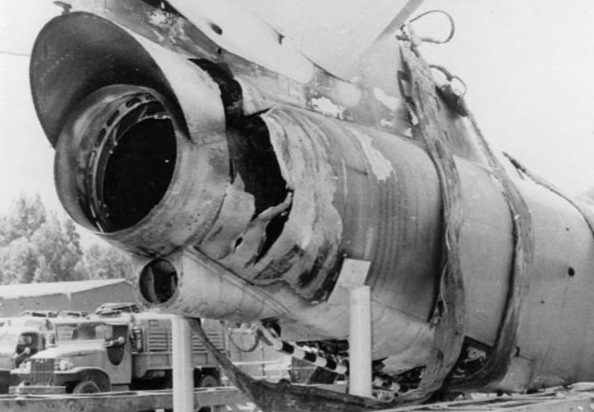
\includegraphics[scale=0.4]{Dolina_4/c8PBnljCPeo.jpg}
	%	\label{fig:scipion} % Unique label used for referencing the figure in-text\end{document}
	%	%\addcontentsline{toc}{figure}{Figure \ref{fig:placeholder}} % Uncomment to add the figure to the table of contents%----------------------------------------------------------------------------------------
	\caption{«Скайхок» №62 Моше Мельника из 115-й эскадрильи, получивший сходные повреждения 19 августа 1969 года. Был отремонтирован и в 1970-м принял участие в боях над Суэцким Каналом}%	CHAPTER 2
\end{figure}

Следующую попытку 27 июля (по израильским данным — 20 июля) предприняли пилоты 135-го ИАП полковника Коротюка. Они избрали несколько иной способ охоты на «Миражи» — что называется, «на живца». В качестве приманки были выбраны египеские МиГ-17. План был простой — египтяне четвёркой атакуют цели на Синае и уходят за Канал. Израильтяне их преследуют, и сталкиваются с советскими пилотами. Вроде просто? Ага, щас. Всё закончилось не сильно хорошо — из-за неразберихи и плохой координации.

Атаку запланировали на 12:00. Египтяне четко выполнили свою часть плана. Советские пилоты — свою, ожидая противника в засаде на малой высоте. Всех подвели израильские лётчики — они просто не явились на бой. Вторая атака в 16:30 также была проведена по графику. Египтяне отбомбились — правда, тут их уже ждали «Миражи». В итоге египтянам удалось уйти за канал, где двух из них сбил лидер пары «Миражей», Ифтах Спектор (обе победы подтверждаются). Самым неприятным было то, что в районе боя, происходившего \textbf{западнее Канала}, уже находилась пара советских самолётов, они (как многие пишут) отлично видели происходящее, но не могли ничего сделать — на советском командном пункте ждали, когда в воздух поднимутся ещё два звена. К моменту их появления всё давно закончилось — «Миражи» уже заходили на посадку в Рефидим.

Сложно сказать, кто ошибся — обе стороны обвиняют друг друга. Одним из египетских пилотов был Мохаммед Заки Окаша, командир эскадрильи МиГ-17 и герой войны 1973 года. Тогда он о советских лётчиках, постоянно обвинявших египтян в трусости и непрофессионализме, отозвался крайне нелицеприятно. Но честно говоря, я могу его понять.

\begin{figure}[h!tb] 
	\centering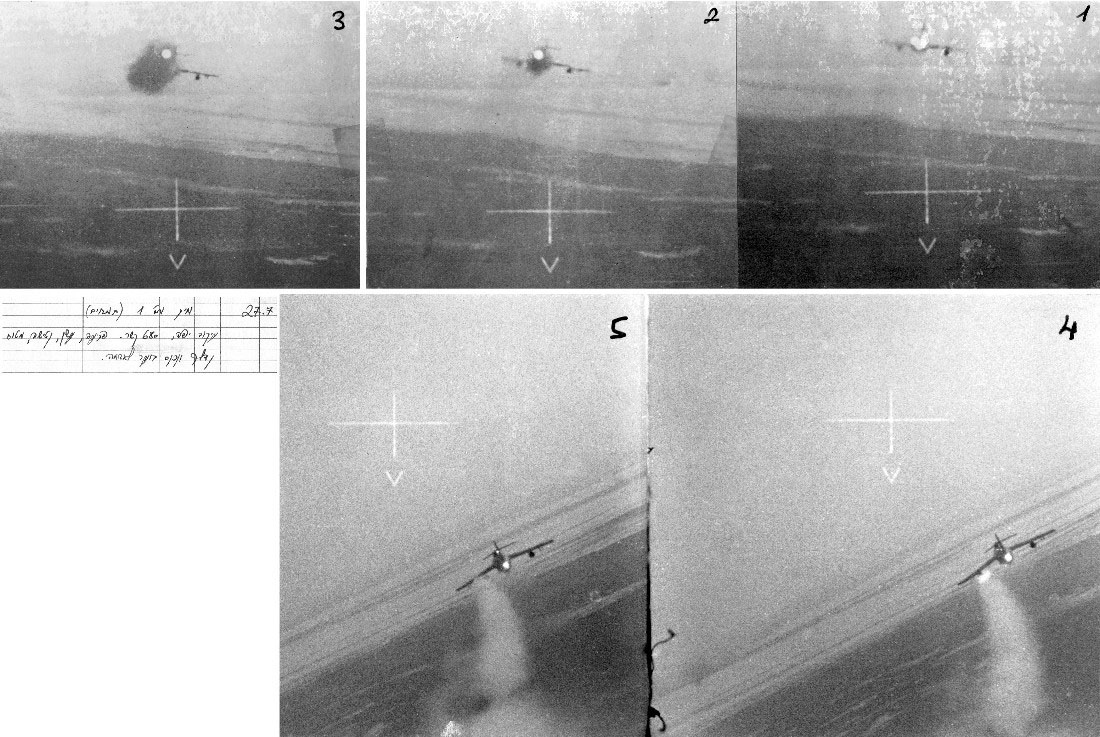
\includegraphics[scale=0.4]{Dolina_4/vw7qFC7JZts.jpg}
	%	\label{fig:scipion} % Unique label used for referencing the figure in-text\end{document}
	%	%\addcontentsline{toc}{figure}{Figure \ref{fig:placeholder}} % Uncomment to add the figure to the table of contents%----------------------------------------------------------------------------------------
	\caption{Кадры ФКП «Миража» Ифтаха Спектора, сбившего два МиГ-17 20 июля 1970 года.}%	CHAPTER 2
\end{figure}
\begin{figure}[h!tb] 
	\centering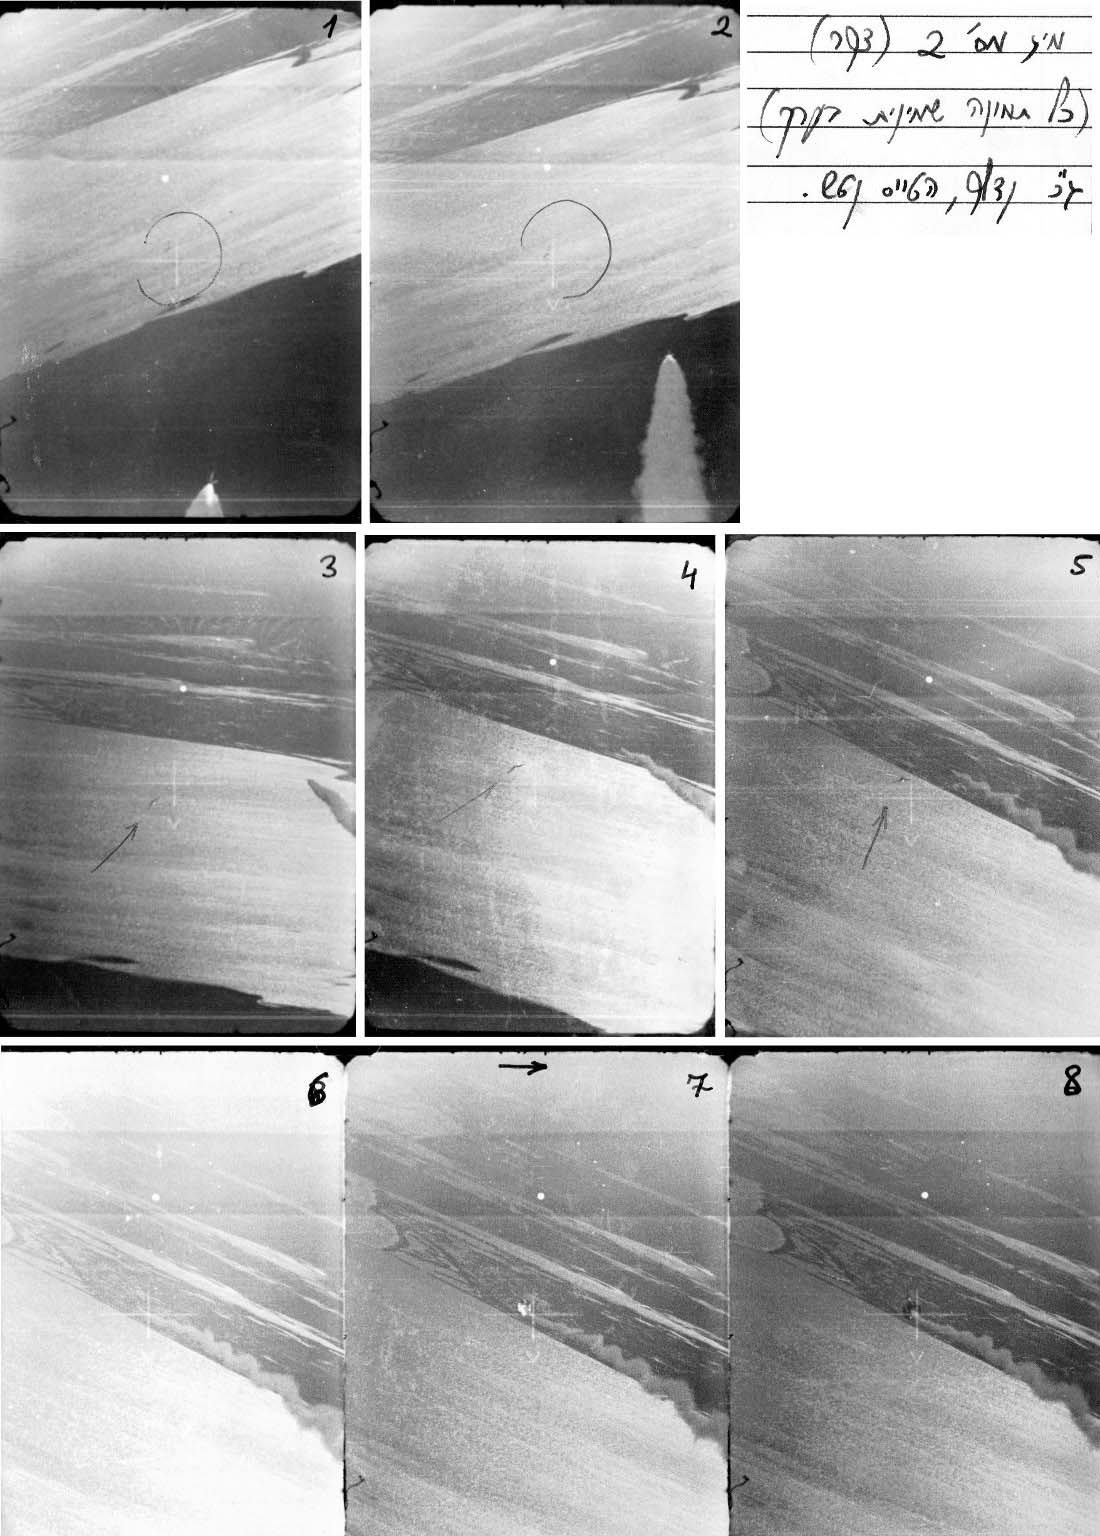
\includegraphics[scale=0.4]{Dolina_4/DPeAH3iJCp8.jpg}
	%	\label{fig:scipion} % Unique label used for referencing the figure in-text\end{document}
	%	%\addcontentsline{toc}{figure}{Figure \ref{fig:placeholder}} % Uncomment to add the figure to the table of contents%----------------------------------------------------------------------------------------
	\caption{Кадры ФКП «Миража» Ифтаха Спектора, сбившего два МиГ-17 20 июля 1970 года.}%	CHAPTER 2
\end{figure}

После этого эпизода советско-египетские отношения, и так не самые лучшие, начали окончательно давать трещину. Речь не только о политиках — египетские пилоты испытывали к своим советским коллегами не самые приятные чувства. Советники от ВВС нередко вели себя высокомерно, и теперь они сами показали себя не лучшим образом.

Тем временем в Израиле. В апреле 1970 года, Голда (Меир, премьер-министр Израиля) на совещании в Кирье произнесла в отношении СССР знаменитую фразу: «Допустим, самолет ВВС Израиля сбивает МиГ, пилотируемый русским. Я не буду довольна в этот день. В любом случае, СССР это большой гой. Это не Египет и не Сирия. \textbf{Я не буду довольна если мы собьем русского}». В слове «гой» в случае Голды нет негативной коннотации, для неё «гой» — это чужак. Советский Союз — страна чуждая, и могущая доставить множество проблем.

В конце июля были обнаружены попытки передвинуть советские дивизионы ЗРК к Каналу, а в приканальной зоне израильская разведка постоянно перехватывала переговоры пилотов МиГов и их КП, тоже на русском. Всё это с точки зрения израильтян говорило только об одном: великая красная сверхдержава решила окончательно связать Израилю руки. Выбора не было, дальнейшее отступление из зоны Канала для израильтян было равносильно поражению в войне.

А для арабов — признанием того, что Израиль можно победить, что Израиль можно изнурить, что он слаб, что Насер выбрал правильную тактику. В тот момент столкновение с советскими лётчиками стало неизбежным. Более того, оно стало вопросом выживания. Решение о планировании операции, целью которой станут именно советские лётчики было тяжелым и драматичным, с многочисленными дискуссиями. Окончательное решение было принято 25 июля, после упомянутой выше атаки на «Скайхок» над каналом. Мордехай Ход и его штаб получили задачу спланировать операцию против советских лётчиков. Отсчёт начался.

\subsection{Масрега}

На исход боя оказало очень большое влияние ещё одно маленькое, но очень важное подразделение. Дело в том, что после появления огромного советского контингента советников в Египте, израильская военная разведка, АМАН, создала наконец «русский» отдел. Назвали его «Масрега» — «спица» на иврите. Название не несло смысловой нагрузки — его просто взяли из банка названий. В быту их чаще называли «гречкоим» — в честь министра Обороны СССР.

Именно они первыми подтвердили 18 апреля 70-го, что русские лётчики над Египтом — уже не советники, а боевые пилоты на задании. Именно они подтвердили, что «Скайхок» над Каналом был атакован советским лётчиком. Именно они прослушивали каналы радиосвязи советских эскадрилий, зная каждого лётчика по голосу. В бою 30 июля «гречки» сыграют ключевую роль — но об этом ниже.

Здесь отметим ту пропасть, которая была между информированностью израильтян и советских военнослужащих. Израильтяне к лету 70-го различали советских пилотов по голосу, по именам. Умели распознавать высоту полёта по тому, как звучит голос лётчика в разреженной атмосфере. Узнали много об отношениях между пилотами, их настроении. В Каире об этом знали, и периодически взлетали в радиомолчании — отчасти, это помогало.

Советский же пилот знал о своих противниках примерно ничего. Ещё в Союзе им рассказали о том, что ВВС Израиля комплектуются из … наёмников (привет, парни, ваши знания устарели на 20 лет), и представляют собой «элитную» 101-ю эскадрилью и множество других, вспомогательных. Судя по всему, ни об уникальной школе ВВС, ни об осмыслении колоссального объёма и опыта воздушных боёв они не знали.

Я не знаю, как это можно назвать. Раздолбайством, помноженным на тотальную секретность. В Союзе, похоже, были уверены, что «Мокед» придумали и проделали лётчики-наёмники, собранные по всему миру. Что их арабских протеже сбивают в соотношении 12:1 наёмники. Постоянно говорится про некий «вьетнамский опыт» — при этом никто толком не может объяснить, в чём он заключался. Я не могу сказать, что послужило причиной такого отношения.

Полковник Борис Абрамов (представитель от управления ПВО и Авиации ГШ в оперативной группе «Кавказ»):

\begin{textcitation}
	Среди рядового и руководящего состава нашей авиационной группы царила излишняя самоуверенность, кое у кого переходящая в шапкозакидательство.
\end{textcitation}

\textbf{Но я уверен, что это высокомерие, это нежелание понимать своего противника, инертность мышления, снисходительность — сыграли свою роль в итоговом результате.}

\subsection{Если попадёте в плен — мы вас не знаем}

Советские пилоты оказались в весьма двусмысленном положении, некоторого рода «лётчиками Шрёдингера». Согласно официальной советской пропаганде того времени, их просто не существовало. Суть проблемы во время проводов офицеров в Египет с восхитительной точностью и прямотой передал министр обороны Гречко: \textbf{«Имейте в виду, товарищи, если вас собьют за Суэцким каналом, и вы попадете в плен — мы вас не знаем, выкарабкивайтесь сами»}. Справедливости ради, я не нашел первоисточника этой фразы, но её повторяет такое огромное количество участников командировки, что в её достоверности я не сомневаюсь.

И правда, что бы делал советский лётчик, попади он в плен? Вероятно, мог попытаться прикинуться арабом… первые минут десять. Всё это ставило в очень двусмысленное положение, как когда-то пилотов МиГ-15 в Корее, которым фактически запрещалось пересекать тридцать восьмую параллель. Олег Цой, Герой России, знаменитый лётчик — испытатель, а в те годы — пилот 135-го ИАП в Египте, сформулировал ещё проще:  \textbf{«Для такого случая у каждого летчика был с собой пистолет и 4 магазина к нему…»}.

Мёртвый русский пилот очень слабо отличается от мёртвого восточного немца.

Но не будем о грустном. 

\subsection{Подготовка к операции}

25 июля премьер-министр Израиля одобрила подготовку операции против советских лётчиков. К тому моменту израильтяне уже успели несколько раз столкнуться с советской «ракетной стеной», разместившейся к западу от Канала, и не сказать, чтобы эти встречи были для них успешными. Было потеряно уже четыре «Фантома», без достигнутых успехов. При этом израильтяне работали на пределе, испробовав все возможные тактики: налёты проводились лучшими лётчиками, с использованием американских средств РЭБ, демонстративных групп, пассивных помех, «звездой», то есть атакующие самолёты заходили на цель с разных сторон. Это было тяжелым испытанием для советских солдат — но «ракетный щит» устоял.

Операцию «Римон-20» изначально запланировали на 29 июля, позже перенеся на 30 число. С самим названием связано несколько мифов. Число 20 является не более, чем кодовым номером. «Римоны» («гранаты», «римоним» на иврите) - серия воздушных боёв, прошедших в середине 69го года. «Римон-20» был ещё одним.

Суть операции сводилась к следующему. Группа «Фантомов» 69-й эскадрильи атакует радарную станцию в районе Суэца. При этом они маскируются под «Скайхоки» — то есть заходят на цель медленно, строятся в круг, и бомбят со средних высот, не заходя в область поражения ствольной артиллерии. Со стороны это должно было выглядеть как очередная рутинная атака, не более. В то же время четвёрка «Миражей» 119-й эскадрильи в плотном строю имитирует разведывательный полёт на большой высоте. Предполагалось, что отметки самолётов «сольются», и на радаре они будут выглядеть, как пара фоторазведки. К тому же, для полноты маскировки, радиообмен должны были вести те лётчики четвёрки, которые раньше уже летали в такие разведывательные вылеты. 

\begin{figure}[h!tb] 
	\centering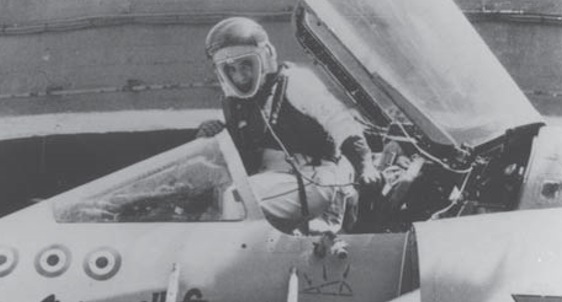
\includegraphics[scale=0.4]{Dolina_4/PV0i3RbdiKE.jpg}
	%	\label{fig:scipion} % Unique label used for referencing the figure in-text\end{document}
	%	%\addcontentsline{toc}{figure}{Figure \ref{fig:placeholder}} % Uncomment to add the figure to the table of contents%----------------------------------------------------------------------------------------
	\caption{«Мираж» №78 из 119-й эскадрильи и пилот в костюме для высотных полётов. 30 июля 1970 года на Авраам Салмон одержит на нём 1,5 победы. Также, эскадрилья имела два специализированных фоторазведчика (98 и 99)}%	CHAPTER 2
\end{figure}

Расчет был на то, что советские пилоты взлетят на перехват если не «Скайхоков» у канала, то хотя бы «Миражей» практически у них над головой.

Третье и четвёртое израильское звено из 101-й и 117-й эскадрилий должны были соответственно дежурить в полной боевой готовности в Рефидим и на малой высоте в районе Суэцкого залива, чтобы иметь возможность быстро вмешаться в ход боя, на случай непредвиденных осложнений. Забегая вперёд — они практически не успеют принять участие в бою.

Как выбирали пилотов для этой операции? Очень просто. От каждой из трёх эскадрилий «Миражей» предложили выставить по звену. Разумеется, в него каждый из трёх комэсков назначил себя, своего зама, и ещё пару пилотов, которых он счёт подходящими для такого задания.

От «Фантомов» требовалось одно звено — его «обеспечила» одна из двух эскадрилий этих самолётов в ВВС, 69-я. 201-я не участвовала — вероятно, это было связано с гибелью её командира, Шмуэля Хеца, во время боя с советским ПВО неделей ранее. Хеца заменил Ран Ронен (Пекер), никогда на «Фантоме» не летавший — разумеется, он, при всём колоссальном опыте, не был лучшим кандидатом для такой задачи.

План был простой: советские лётчики поднимаются для перехвата «Скайхоков», видят «Миражи», атакуют их. В это время они сами оказываются атакованы четвёркой «Фантомов» с малой высоты, и в идеальном для израильтян положении — советские самолёты должны были находиться на фоне неба, не маневрируя. Лёгкая цель для «Спэрроу» и минимум риска. Правда, бой прошёл не совсем по такому сценарию, но об этом чуть ниже.

\subsection{30 июля 1970 года, утро}

«Римон-20» был, без сомнения, важной операцией, но далеко не единственной. Египетские РЛС и артиллерийские батареи сами себя на разбомбят — так что с утра пары и четверки эскадрилий «Фантомов», «Скайхоков», старых «Вотуров» и «Ураганов» продолжили свой рутинный путь к целям на западном берегу Канала. Они не встретили серьёзного сопротивления — только дежурный, слабый огонь ПВО. Всё самое интересное осталось на вторую половину дня. Банк целей опустел — так что пришло время положить сыр в мышеловку.

Египтяне, к слову, не оставались в долгу. С 30 июня по 15 июля они 11 раз атаковали позиции израильских «Хоков», добившись нескольких попаданий.

Итак, 30 июля приблизительно в 15:00 по египетскому времени и 14:00 по израильскому, стартовала знаменитая операция «Римон-20». Целью израильской стороны было нанесение максимального урона советским ВВС в Египте. У советской стороны конкретной цели не было — они об операции против них просто не знали.

Основные участники мероприятия:

СССР:

\begin{itemize}
	\item Вынесенный командный пункт авиации в Бир-Арейда (Дольников, Мубарак, по другой версии, они находились в Каире)
	\item КП 135 истребительного авиаполка на аэродроме Ком-Аушим
	\item Советские самолёты 135-го ИАП базировались на двух основных аэродромах - Бени-Суэф (1-я и 2-я эскадрилья)и Ком-Аушим (3-я эскадрилья). Непосредственно в бою участвовали два звена 2-й и 3-й эскадрильи. Ещё одно звено второй эскадрильи появилось в районе боя до его завершения, но никакого участия в нем не приняло. Итак:
	\item Звено 3-й эскадрильи из Ком-Аушим (вступило в бой первым, далее - «звено Каменева») — Каменев, ???, ???, Журавлев (погиб). 
	
	\begin{figure}[h!tb] 
		\centering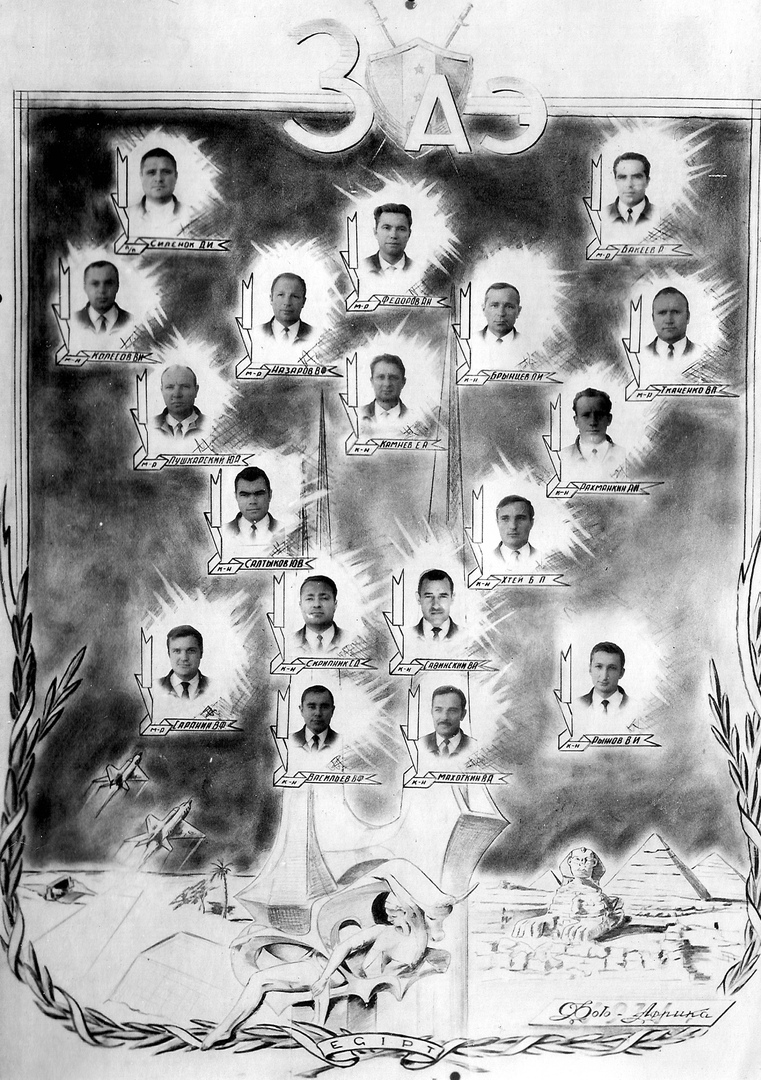
\includegraphics[scale=3.0]{Dolina_4/Y7omxATdv0k.jpg}
		%	\label{fig:scipion} % Unique label used for referencing the figure in-text\end{document}
		%	%\addcontentsline{toc}{figure}{Figure \ref{fig:placeholder}} % Uncomment to add the figure to the table of contents%----------------------------------------------------------------------------------------
		\caption{Коллективное фото лётчиков 3-й эскадрильи, фото с сайта hubara-rus}%	CHAPTER 2
	\end{figure}
	\item Звено 2-й эскадрильи из Бени-Суэф (вступило в бой вторым, далее - «звено Юрченко») — Юрченко (замкомэска, погиб), Макара (начштаба эскадрильи, аварийная посадка), Сыркин (катапультировался), Яковлев (погиб).
	
	\begin{figure}[h!tb] 
		\centering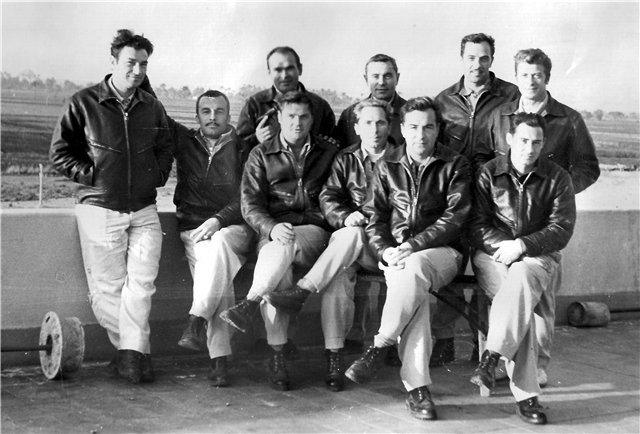
\includegraphics[scale=0.4]{Dolina_4/C66R0acj3xk.jpg}
		%	\label{fig:scipion} % Unique label used for referencing the figure in-text\end{document}
		%	%\addcontentsline{toc}{figure}{Figure \ref{fig:placeholder}} % Uncomment to add the figure to the table of contents%----------------------------------------------------------------------------------------
		\caption{Фото лётчиков 2-й эскадрильи. Второй слева — Сыркин, (из личного архива Васильева, с сайта hubara-rus)}%	CHAPTER 2
	\end{figure}
	\begin{figure}[h!tb] 
		\centering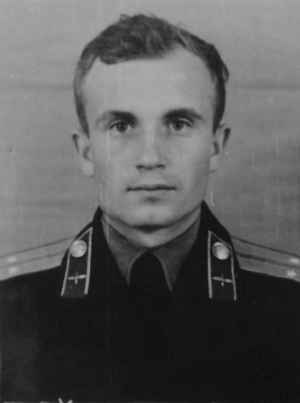
\includegraphics[scale=0.4]{Dolina_4/7KipCSMMz64.jpg}
		%	\label{fig:scipion} % Unique label used for referencing the figure in-text\end{document}
		%	%\addcontentsline{toc}{figure}{Figure \ref{fig:placeholder}} % Uncomment to add the figure to the table of contents%----------------------------------------------------------------------------------------
		\caption{Капитан Е.Г. Яковлев из пары Тираспольского авиаполка:}%	CHAPTER 2
	\end{figure}
	\begin{figure}[h!tb] 
		\centering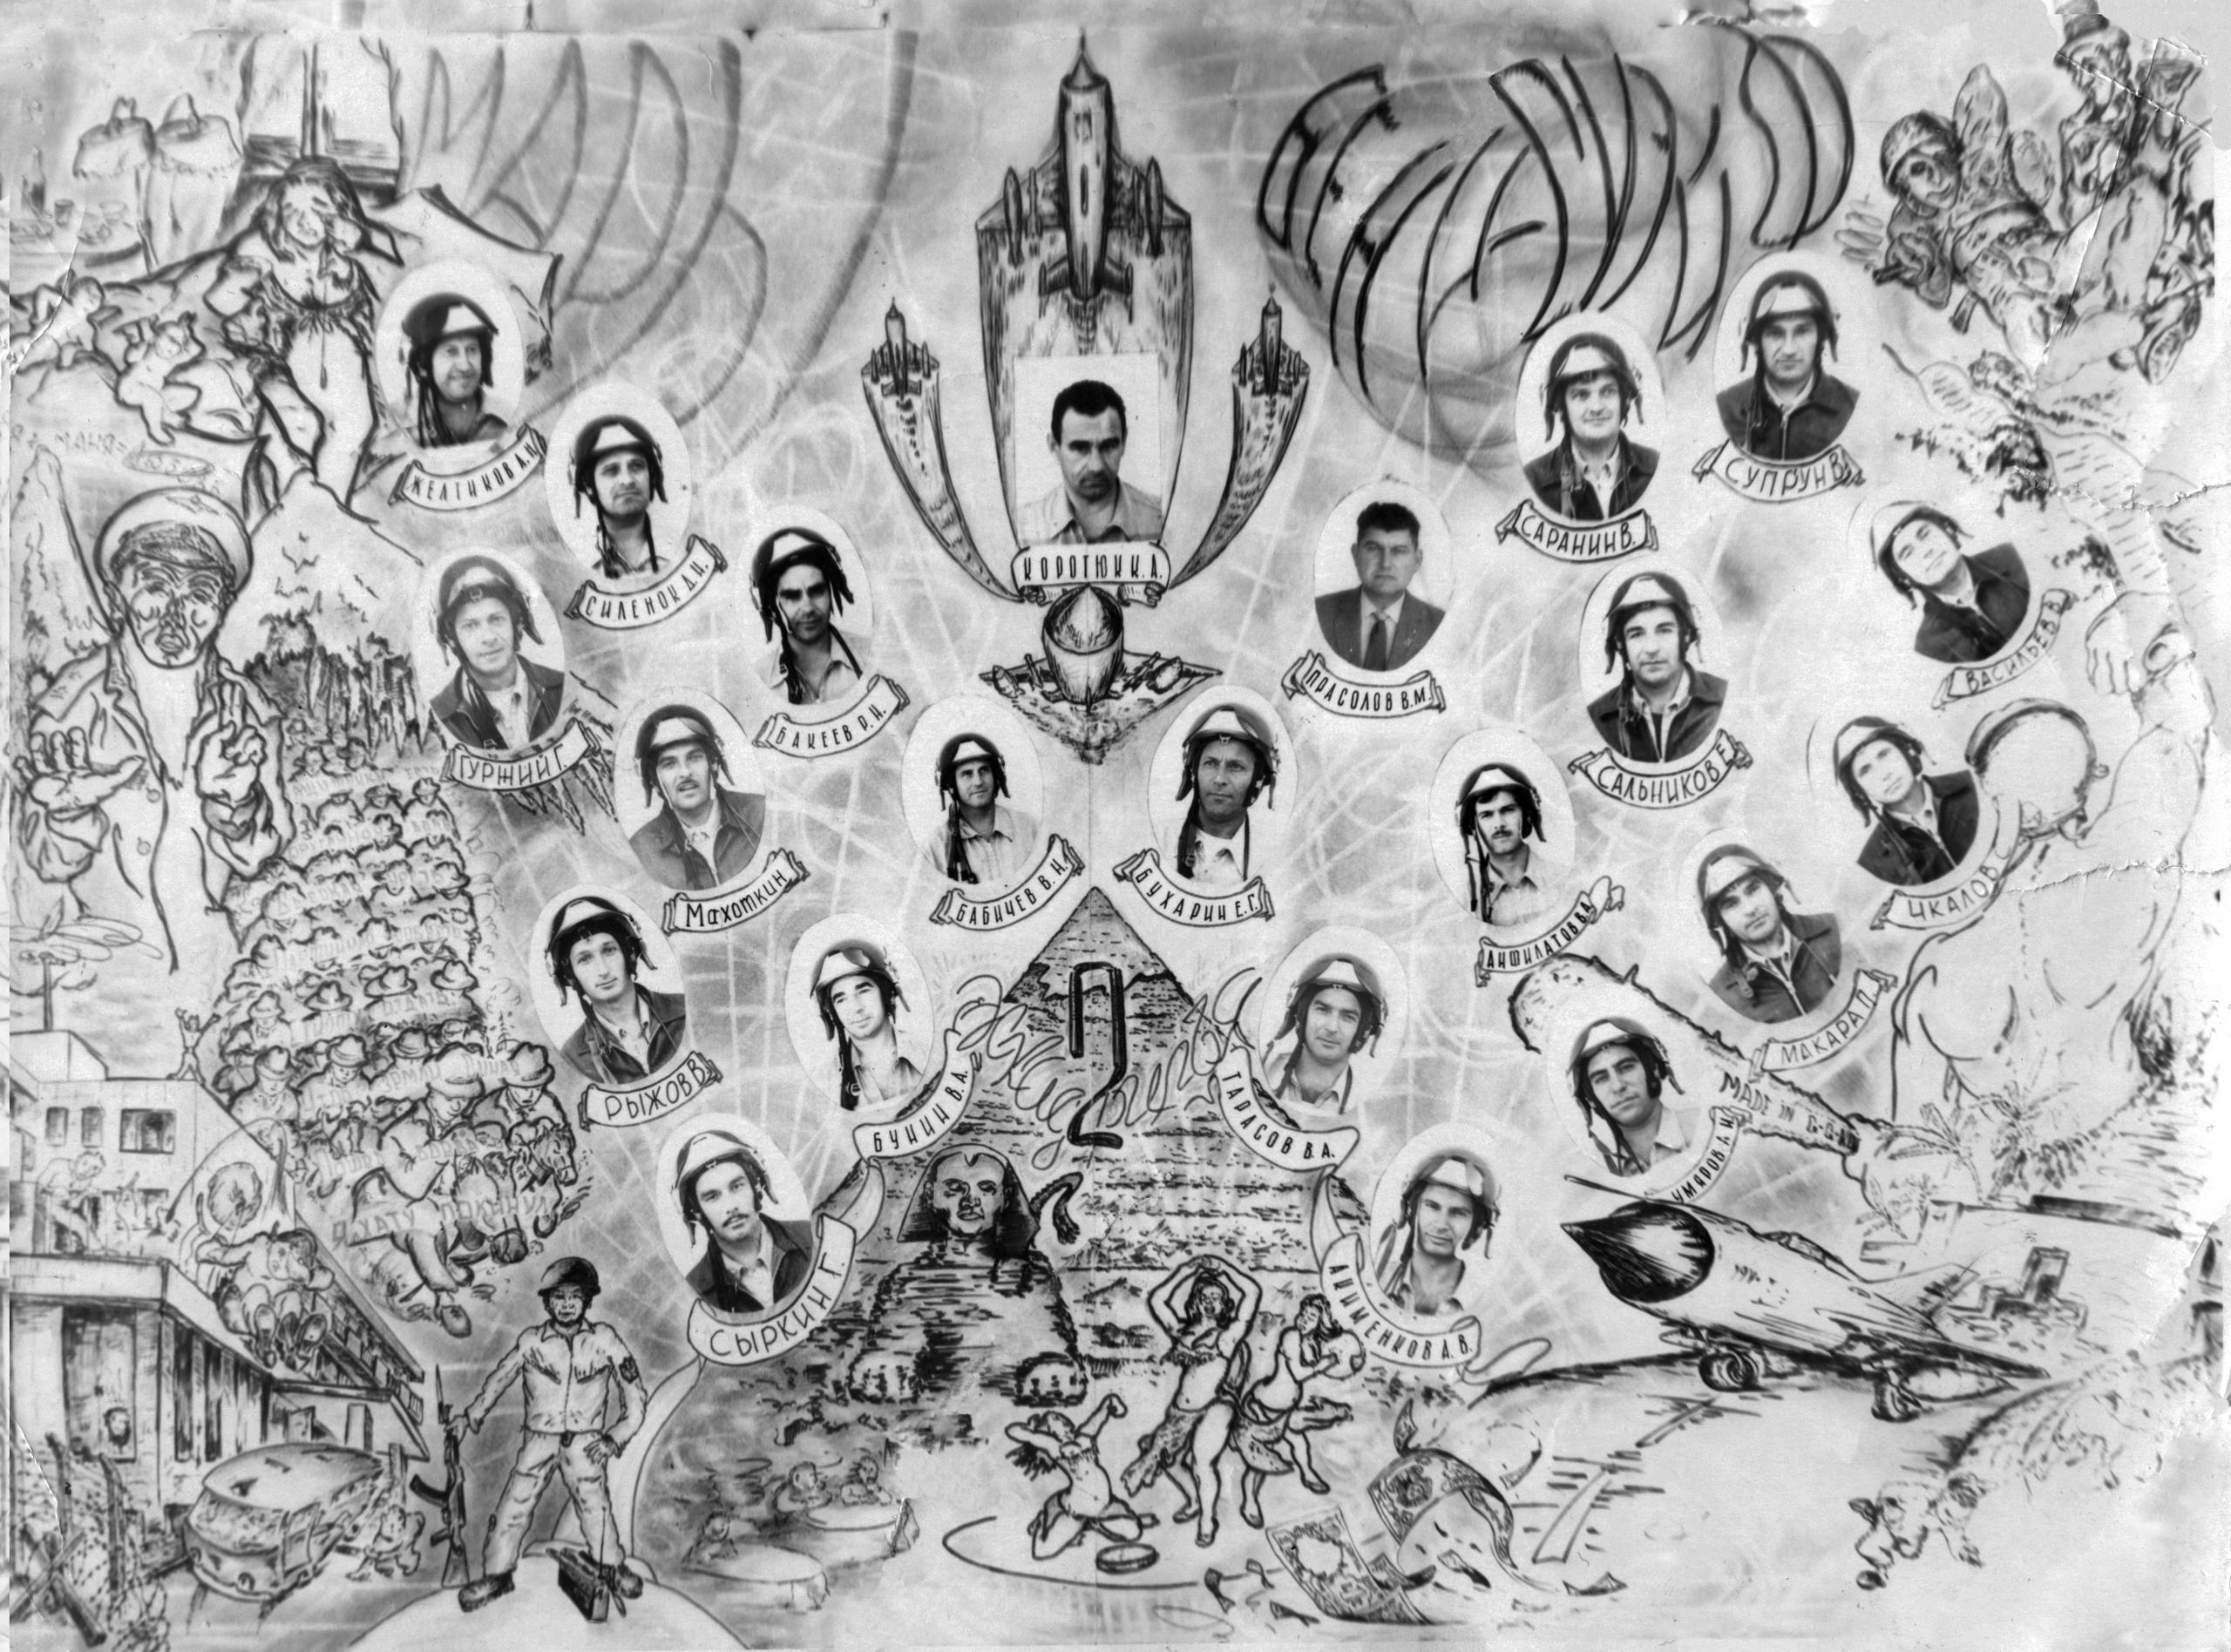
\includegraphics[scale=0.4]{Dolina_4/9wC9C0-AuGw.jpg}
		%	\label{fig:scipion} % Unique label used for referencing the figure in-text\end{document}
		%	%\addcontentsline{toc}{figure}{Figure \ref{fig:placeholder}} % Uncomment to add the figure to the table of contents%----------------------------------------------------------------------------------------
		\caption{Коллективное фото 2-й эскадрильи:}%	CHAPTER 2
	\end{figure}
	\item Звено 2-й эскадрильи из Бени-Суэф (фактически, не участвовало в бою, но находилось в том районе, далее — «звено Саранина») — Саранин, Васильев, Супрун, Мазур.
	\begin{figure}[h!tb] 
		\centering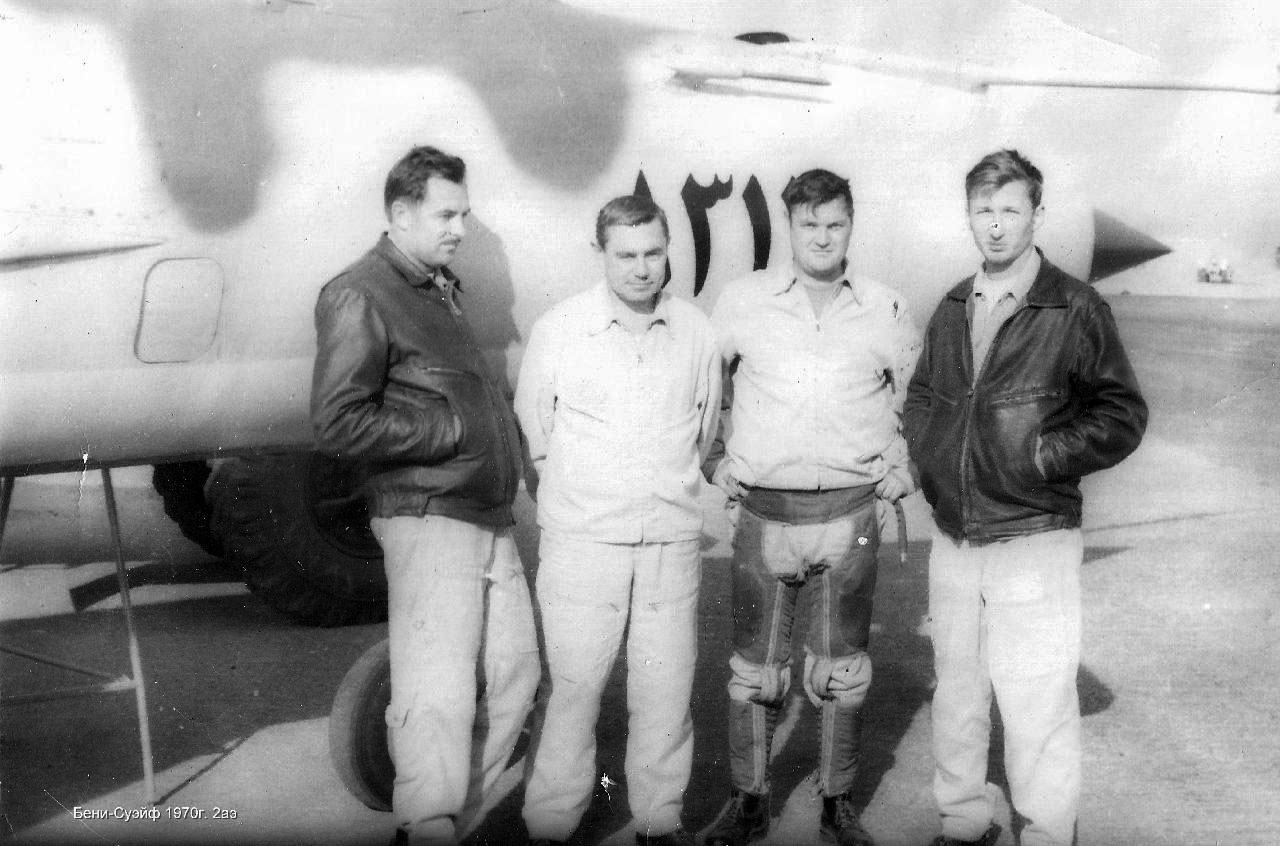
\includegraphics[scale=0.4]{Dolina_4/guazHS_eHMc.jpg}
		%	\label{fig:scipion} % Unique label used for referencing the figure in-text\end{document}
		%	%\addcontentsline{toc}{figure}{Figure \ref{fig:placeholder}} % Uncomment to add the figure to the table of contents%----------------------------------------------------------------------------------------
		\caption{Дежурное звено Саранина, Слева направо: В.А. Махоткин, В.Ф. Васильев, В.Ф. Саранин, В.И. Рыжов МиГ-21 (бортовой №831... (8311, 8312, 8313 ?)). 135 иап. Ком-Аушим. (из личного архива В.Ф. Васильева). Фото с сайта hubara-rus}%	CHAPTER 2
	\end{figure}
	\item Все остальные советские самолёты (пара из Котмии, два звена с Бени-Суэф и Ком-Аушим) появились в воздухе достаточно поздно, а в районе боя были уже сильно после его окончания.
\end{itemize}

Общее командование — генерал-лейтенант Г.У. Дольников.

Тут был ещё один момент. По воспоминаниям советских лётчиков (конкретно, Васильева, которые известны со слов его сына на http://forums.airbase.ru), у советской стороны большой сложностью были проблемы со здоровьем личного состава. Так, разбивались привычные звенья, пришедшие из одних полков— к примеру, «тираспольское» звено Яковлев-Сыркин-Махоткин-Рыжов в тот раз взлетело в составе Юрченко-Макара-Яковлев-Сыркин.

К сожалению, фото большинства советских участников того боя в открытых источниках не доступны.

Израиль:
\begin{itemize}
	\item Четвёрка «фоторазведчиков» — «Миражей» из 119-й эскадрильи (далее — «разведчики»). Амос Амир (комэск), Ашер Снир, Авраам Салмон, Ави Гилад. Именно это звено вместе с «Фантомами» из 69-й было основным участником боя с израильской стороны.
	\begin{figure}[h!tb] 
		\centering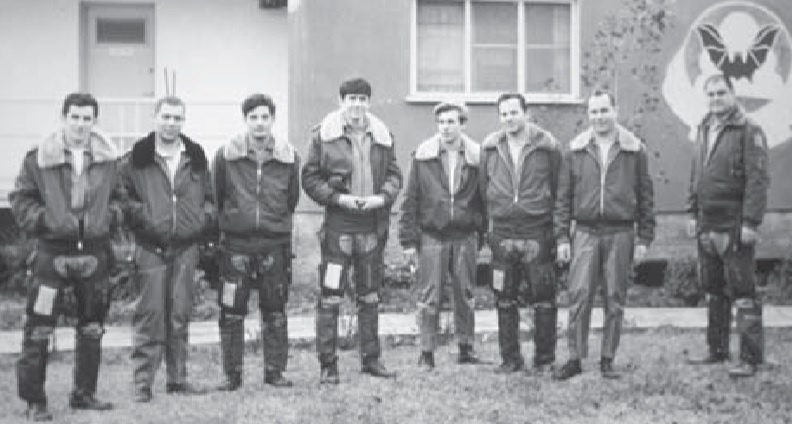
\includegraphics[scale=0.4]{Dolina_4/FWa94mCdeK8.jpg}
		%	\label{fig:scipion} % Unique label used for referencing the figure in-text\end{document}
		%	%\addcontentsline{toc}{figure}{Figure \ref{fig:placeholder}} % Uncomment to add the figure to the table of contents%----------------------------------------------------------------------------------------
		\caption{119-я эскадрилья (неполный состав). Слева-направо: Ашер Снир (младший замкомэска), Ицик Нир, Мики Кац, Ави Гилад, Амос Шахар, Авраам Салмон (старший замкомэска), Амос Амир (комэск), Реувен Розен. 53 сбитых на 8 человек, в тот момент. Фото из книг Шломо Алони}%	CHAPTER 2
	\end{figure}
	\item Четвёрка «Миражей» из 117-й эскадрильи (далее — «звено 117-й»). Ури Эвен-Нир, Итамар Нойнер, Коби Рихтер, Эхуда Корен. Выполняли роль «усиления», взлетели незадолго до начала боя и находились ниже радиогоризонта на малой высоте. Перед началом боя первая пара (Эвен-Нойнер) вернулась на аэродром по техническим причинам, у командира эскадрильи возникли проблемы с двигателем. Вторая пара звена приняла ограниченное участие в преследовании уходящих советских лётчиков.
	\item Четвёрка «Миражей» из 101-й эскадрильи (далее — «звено Спектора»). Йифтах Спектор, Михаэль Цук, Исраэль Бахарав, Гиора Рам. Первая пара звена поднялась в воздух в момент начала боя и приняла участие в преследовании советских лётчиков, Спектор даже записал себе одну победу (тот самый спорный пятый сбитый МиГ, об этом подробно ниже). Вторая пара в бою не участвовала. 
	\begin{figure}[h!tb] 
		\centering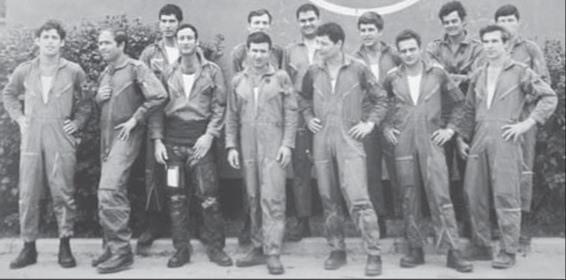
\includegraphics[scale=0.4]{Dolina_4/4ynJzvFshYY.jpg}
		%	\label{fig:scipion} % Unique label used for referencing the figure in-text\end{document}
		%	%\addcontentsline{toc}{figure}{Figure \ref{fig:placeholder}} % Uncomment to add the figure to the table of contents%----------------------------------------------------------------------------------------
		\caption{101-я эскадрилья (неполный состав). Слева-направо первый ряд: Геба, Хабер, Север, Эпштейн, Спектор, Цук, Шахар. Второй ряд: Авербух, Дрор, Розен, Яари, Карми, Хертц. 80.5 побед на 13 человек в тот момент. Фото из книг Шломо Алони}%	CHAPTER 2
	\end{figure}	
	\item     Четвёрка «Фантомов» 69-й эскадрильи (далее — «Фантомы»). Авиху Бин-Нун+Шауль Леви, Авием Селла+Реувен Решеф (Фишер), Эхуд Ханкин+???, Ури Гиль+Исраэль Парнас. Планировалось, что это звено атакует советские самолёты, преследующие «разведчиков», из наиболее удобного для себя положения — захватив цель радаром, на фоне неба. Фактически, они были вынуждены вместо этого участвовать в манёвренном бою с МиГами, и преуспели в этом.
	
	\item Подразделения РЭБ и РТР на Синае.
\end{itemize}

Общее командование — главком ВВС Израиля Мордехай Ход.

У израильтян проблемы со слётанностью звеньев в принципе практически не было — там считалось нормальным всем летать со всеми. Тем более, имеющаяся система с наличием большого количества лётчиков-резервистов, находящихся в эскадрилье непостоянно, этому способствовала…
